% Windows: протестировано для MikTeX+TeXworks в режиме pdfLatex.
%
% Linux:
% Для получения pdf используйте команду  pdflatex rfa_2021.tex.
% Команда latex rfa_2021.tex выведет сообщение об ошибке.
%
\NeedsTeXFormat{LaTeX2e}
\documentclass[10pt,a4paper]{book}
\usepackage{NumMet_2022}
%--- Здесь можно вставить необходимые стили ---
% \usepackage{...}
%
%--- Здесь можно добавить свои команды --------
% \newcommand{}
\newcommand{\ceq}{\mathrel{\vcenter{\hbox{:=}}}}
%----------------------------------------------
\selectlanguage{russian}
\begin{document}
%===========================  ШАПКА СТАТЬИ =================================
\Article{О реализации параллельного алгоритма глобальной оптимизации с использованием набора инструментов Intel oneAPI
}%Обновить перевод названия
    {Solving time-consuming multidimensional global optimization problems with Intel OneApi tools}
    
\Abstract{В статье рассматривается параллельный алгоритм решения задач глобальной оптимизации и обсуждается его реализация с использованием набора инструментов Intel oneAPI. Предполагается, что целевая функция задачи задана как <<черный ящик>> и удовлетворяет условию Липшица. Изложенный в статье параллельный алгоритм использует схему редукции размерности на основе кривых Пеано, которые непрерывно и однозначно отображают отрезок вещественной оси на гиперкуб.
В качестве средства для реализации параллельного алгоритма использован инструментарий Intel oneAPI, который позволяет писать один код как для центрального процессора, так и для графических ускорителей. Приведены результаты вычислительных экспериментов, полученные при решении серии сложных задач многоэкстремальной оптимизации.}
%обновить перевод - сейчас он для старой аннотации
    {The paper considers the process of solving a series of time-consuming global optimization problems. We suppose that the objective function satisfies the Lipschitz condition with a priory unknown Lipschitz constant. Intel OneApi tools, that allows one to write the same code for both the central processor and the graphics accelerator, are chosen for implementing the parallel global optimization algorithm. To solve multidimensional problems, we use an approach based on the idea of dimensionality reduction using the Peano curve, which continuously maps an interval of the real axis onto an n-dimensional cube.}

\Keywords{глобальная оптимизация,
многоэкстремальные функции,
параллельные вычисления,
редукция размерности,
графические ускорители,
Intel OneAPI.}
        {global optimization,
multiextremal functions,
parallel computing,
reduction of dimensionality,
graphics accelerators,
Intel OneApi.}

\Acknowledgements{Работа выполнена при поддержке программы Центра компетенций OneAPI в ННГУ, Министерства науки и высшего образования РФ (проект № 0729-2020-0055) и научно-образовательного математического центра «Математика технологий будущего» (проект № 075-02-2021-1394).}
    {Работа выполнена при поддержке программы Центра компетенций OneAPI в ННГУ, Министерства науки и высшего образования РФ (проект № 0729-2020-0055) и научно-образовательного математического центра «Математика технологий будущего» (проект № 075-02-2021-1394).}

\Citation{Баркалов К.А., Лебедев И.Г., Силенко Я.В.
    Решение трудоемких задач многомерной глобальной оптимизации с использованием набора инструментов Intel oneAPI~//
    Вычислительные методы и программирование. 2022.
    \textbf{??}, \No~?. \pageref*{firstPage}--\pageref*{LastPage}.  
    doi 10.26089/NumMet.v??r???.}
    {K.~A.~Barkalov, I.~G.~Lebedev, Ya.~V.~Silenko,
    Solving time-consuming multidimensional global optimization problems with Intel OneApi tools 
    for the journal ``Numerical methods and programming,''
    Numerical Methods and Programming. \textbf{??} (?), 
    \pageref*{firstPage}--\pageref*{LastPage} (2022).
    doi~10.26089/NumMet.v??r???.}


\UDC{<указывает автор>}
\DOI{10.26089/NumMet.v??r???}% заполняет редакция
\VOL{??}{?}
\YEAR{2022}
\Received{16 июня 2022 г.}{June 16, 2022}
\Accepted{13 октября 2022 г.}{October 13, 2022}



\Author{К.~А.~Баркалов}{Konstantin~A.~Barkalov}
\FullName{Баркалов Константин Александрович}{Konstantin~A.~Barkalov}
% Место работы 1
\Institution{Нижегородский государственный университет им. Н.И. Лобачевского}
{Nizhny Novgorod State University N.I. Lobachevsky}
\Address{пр. Гагарина, д. 23.}{Gagarin Ave., 23.}
\Postcode{603022}
\City{Нижний Новгород}{Nizhny Novgorod}
\CountryOfResidence{Российская Федерация}{Russia}
\AcademicDegree{
Доктор технических наук}{Ph.D.}
\Position{доцент}{docent}
\Orcid{0000-0001-5273-2471}
\Email{konstantinbarkalov@yandex.ru}



\Author{И.~Г.~Лебедев}{Ilya~G.~Lebedev}
\FullName{Лебедев Илья Генадьевич}{Ilya~G.~Lebedev}
% Место работы 1
\Institution{Нижегородский государственный университет им. Н.И. Лобачевского}
{Nizhny Novgorod State University N.I. Lobachevsky}
\Address{пр. Гагарина, д. 23.}{Gagarin Ave., 23.}
\Postcode{603022}
\City{Нижний Новгород}{Nizhny Novgorod}
\CountryOfResidence{Российская Федерация}{Russia}

\Position{заведующий лабораторией}{head of laboratory}
\Orcid{0000-0002-8736-0652}
\Email{ilya.lebedev@itmm.unn.ru}

\Author{Я.~В.~Силенко}{Yanina~V.~Silenko}
\FullName{Силенко Янина Вадимовна}{Yanina~V.~Silenko}
% Место работы 1
\Institution{Нижегородский государственный университет им. Н.И. Лобачевского}
{Nizhny Novgorod State University N.I. Lobachevsky}
\Address{пр. Гагарина, д. 23.}{Gagarin Ave., 23.}
\Postcode{603022}
\City{Нижний Новгород}{Nizhny Novgorod}
\CountryOfResidence{Российская Федерация}{Russia}
\Position{лаборант}{laboratory assistant}
\Orcid{???}
\Email{yanikolt@gmail.com}





\MakeArticleHeader
%========================= КОНЕЦ ШАПКИ СТАТЬИ ==============================

\pagebreak



\section{Постановка задачи}



Задачи поиска экстремумов многоэкстремальных функций часто возникают в различных областях науки, таких как химия, физика, машиностроение и т.д. 

В рамках данной работы рассматривается задача поиска глобального минимума $y^*$ функции $\varphi(y)$ в гиперинтервале $D$, т.е. 
\begin{equation}
\label{task}
\varphi(y^*)=\min\{\varphi(y):y\in D\}, \; D=\{y\in R^N:a_i\leqslant x_i\leqslant{b_i}, 1\leqslant{i}\leqslant{N}\}.
\end{equation}

Будем предполагать, что информация о структурных свойствах целевой функции $\varphi(y)$ неизвестна, а сама функция задается как <<черный ящик>>, т.е. с помощью некоторого реализованного программно алгоритма вычисления ее значений. Также будем предполагать, что $\varphi(y)$ удовлетворяет Липшица 
\begin{equation}
\label{lip}
|\varphi(y_1)-\varphi(y_2)|\leqslant L\Vert y_1-y_2\Vert,y_1,y_2\in D,0<L<\infty,
\end{equation}
причем константа Липшица $L$ априори неизвестна.

%комментарий про разные способы редукции размерности - ссылки на Сергеева, Жилинскаса

Сведение многомерной задачи (\ref{task}) к одномерной проводится за счет использования редукции размерности при помощи кривой Пеано [\ref{rfa:rulit:lit1}, \ref{rfa:rulit:lit2}] $y(x)$, которая непрерывно и однозначно отображает отрезок вещественной оси $[0,1]$ на $N$-мерный гиперкуб:
\begin{equation}
\label{cube}
\lbrace y\in R^N:-2^{-1}\leqslant y_i\leqslant 2^{-1}, 1\leqslant i\leqslant N\rbrace=\{y(x): 0\leqslant x\leqslant 1\}.
\end{equation}
С использованием отображения $y(x)$ решение исходной задачи сводится к минимизации одномерной функции на отрезке $[0,1]$, т.е.
\begin{equation}
\label{oneDimTask}
\varphi(y^*)=\varphi(y(x^*))=\min\{\varphi(y(x)): x\in [0,1]\}.
\end{equation}
 
Указанный способ редукции размерности обладает следующим важным свойством: сохраняется ограниченность относительных разностей функции , т.е. если в области $D$ функция $\varphi(y)$ удовлетворяла условию Липшица, то на интервале $[0,1]$ функция $\varphi(y(x))$ будет удовлетворять равномерному условию Гельдера
\begin{equation}
\label{holder}
\left|\varphi(y(x_1))-\varphi(y(x_2))\right|\leqslant H{\left|x_1-x_2\right|}^{\frac{1}{N}}, 
 x_1,x_2\in[0,1],
\end{equation}
\begin{equation}
H=4Ld\sqrt{N},d=\max\{b_i-a_i:1\leqslant i\leqslant N\}.
\end{equation}
 
 
Пользуясь этим свойством, можно трактовать исходную задачу (\ref{task}) как задачу минимизации одномерной функции $f\left(x\right)=\varphi\left(y\left(x\right)\right)$, $x\in[0,1]$, удовлетворяющей условию Гельдера. %следующий абзац надо поправить
Факт того, что функция задана как «черный ящик», сокращает число подходящих алгоритмов. 
Для исследования выбран алгоритм глобального поиска [\ref{rfa:rulit:lit3}, \ref{rfa:rulit:lit4}], который является одним из эффективных методов глобальной оптимизации, т.к. при решении многих задач опережает (по числу итераций) другие методы аналогичного назначения [\ref{rfa:rulit:lit5} – \ref{rfa:rulit:lit9}]. Алгоритм глобального поиска относится к классу характеристических алгоритмов оптимизации, хорошо масштабируется и отлично подходит для работы на параллельных вычислительных кластерах. 

\section{Параллельный алгоритм глобального поиска}

В процессе своей работы алгоритм порождает последовательность точек $\{x^k\}$, в каждой из которых проходит вычисление значений минимизируемой функции $f(x^k)$. В дальнейшем будем называть процесс вычисления значения одномерной функции в точке $x^k$ \textit{поисковым испытанием}. Испытание включает в себя также построение образа $y^k=y(x^k)$, а результатом испытания является пара $(x^k,\ z^k=f(x^k))$. Процесс распараллеливания построен таким образом, что при выполнении одной итерации метода одновременно проходят $P\geq1$ испытаний. Обозначим $k(n)$ общее число испытаний, которые были проведены после выполнения $n$ параллельных итераций. 
%текст надо исправить
Приведем последовательность этапов параллельного алгоритма глобального поиска с модифицированием для решения задач с функциями, удовлетворяющими условию Гельдера:
Подготовительный этап. Изначально проводится испытание в произвольной внутренней точке $x^1\in\left[0,\ 1\right].\ $ Когда выполнено $n\geq1$ итераций, и соответствующее им число $k=k(n)$ испытаний в точках $x^i,\ 1\le\ i\le\ k$, то точки $x^{k+1},\ldots,x^{k+P}$ испытаний последующей $(n+1)$ итерации будут определять следующим образом:

 1 этап. Упорядочить по координате точки уже проведенных испытаний и граничные точки:
 \begin{equation}
\label{agp1_sort}
	0=x_0<\ x_1<\ ...\ <x_{k+1}=1,
	\end{equation}
	
2 этап. Вычислить текущее значение $M$, оценивающее неизвестную константу Липшица $L$:
 \begin{equation}
\label{agp2_mu}
	\mu=max\left\{\frac{|z_i-z_{i-1}|}{{{(x}_i-x_{i-1})}^{1/N}},\ i=1,\ldots,k\right\},\ M=\ \left\{\begin{matrix}r\mu,\ \mu>0,\\1,\ \mu=0,\\\end{matrix}\right.\
		\end{equation}

   где $r>1$ заданный параметр метода.
   
3 этап. Найти значение характеристики $R(i)$ для всех интервалов

\begin{equation}
\label{agp3_R1}
R(1)=2\Delta_1-4\dfrac{z_1}{M},R(k+1)=2\Delta_{k+1}-4\dfrac{z_k}{M},
\end{equation}

\begin{equation}
\label{agp3_Ri}
R(i)=\Delta_i+\dfrac{(z_i-z_{i-1})^2}{M^2\Delta_i}-2\dfrac{z_i+z_{i-1}}{M},1<i<k+1,
\end{equation}

   где \(\Delta_i=(x_i-x_{i-1})^\frac{1}{N}\).
   
4 этап.  Упорядочить характеристики $R\left(i\right),\ 1\ \le\ i\ \le\ k+1$ в порядке невозрастания 
\begin{equation}
\label{agp4_R_sort}
	R\left(t_1\right)\geq\ R\left(t_2\right)\geq...\geq\ R\left(t_k\right)\geq\ R(t_{k+1}),\ 
\end{equation}	
	
и выбрать P интервалов с номерами $t_j,\ 1\le\ j\le\ P$, значение характеристики в которых наибольшее.

5 этап. В выбранных интервалах вычислить точки $x^{k+j},\ 1\le\ j\le\ P$ и провести в них новые испытания:

\begin{equation}
\label{agp5_x1}
	x^{k+j}=\frac{x_{t_j}+x_{t_j-1}}{2},\ t_j=1,\ t_j=k+1,
\end{equation}	
	
\begin{equation}
\label{agp4_xi}	
	x^{k+1}=\frac{x_{t_j}+x_{t_j-1}}{2}-sign\left(z_{t_j}-z_{t_j-1}\right)\frac{1}{2r}\left[\frac{\left|z_{t_j}-z_{t_j-1}\right|}{\mu}\right]^N,\ 1<t_j<k+1.
\end{equation}	

Важно отметить, что в рассматриваемых задачах самый трудоемкий и времязатратный этап алгоритма – это вычисление значения функции в точке. Поэтому параллельное вычисление этих значений положительно влияет на скорость работы алгоритма.

Используемые критерии остановки: 

	по длине интервала, как только происходит выполнение условия \(\Delta_{t_j}\leqslant \varepsilon\) хотя бы для какого-то номера $t_j,\ 1\le\ j\le\ P$. Основной критерий остановки, используется в прикладных задачах оптимизации и в тестовых наборах, для которых точка глобального минимума заранее неизвестна. 
	 
	по попаданию в окрестность глобального минимума, $\left|x_{t_j}-\ x^\ast\right|<\varepsilon,\ \ t_j,\ 1\le\ j\le\ P$, где $x^\ast$ -- точка глобального минимума, если ее значение известно. Используется в тестовых задачах, когда $x^\ast$ известна до начала работы алгоритма.
	
Как оценка глобально-оптимального решения рассматриваемой задачи (1) выбираются значения 


\begin{equation}
f_k^*=\min_{1\leqslant i \leqslant k}f(x_i), x_k^*=arg \min_{1\leqslant i \leqslant k}f(x_i).
\end{equation}


\section{Теоретические оценки ускорения параллельного алгоритма}
Опишем (по книге [\ref{rfa:rulit:lit2}]) теоретические свойства параллельного алгоритма. В решаемых задачах время выполнения одного испытания существенно превышает время обработки ее результата. Таким образом, ускорение по испытаниям будет:

\begin{equation} \label{par_trl_ref}
s(p) = \frac{n(1) \cdot p}{n(p)}
\end{equation}

$s(p)$ является ключевой характеристикой эффективности параллельного алгоритма глобального поиска. Где $n(1)$ — количество испытаний, выполненных последовательным алгоритмом, а $n(p)$ — количество испытаний, выполненных параллельным алгоритмом с использованием $p$ параллельных устройств.

Очевидно, что количество испытаний $n(p)$ для алгоритмов с разной степенью распараллеливания $p$ будут отличаться друг от друга. Действительно, последовательный алгоритм имеет полную информацию, полученную на предыдущих $k$ итерациях, при выборе точки $x^{k+1}$ следующего $(k+1)-ого$ испытания. Параллельный алгоритм выбирает не одну, а $p$ точек $x^{k+j}$, $1 \leq j \leq p,$ на основе той же информации. Это означает, что выбор точек $x^{k+j}$ производится без информации о результатах испытаний в точках $x^{k+i}$, $1 \leq i < j$. Только первая точка $x^{k+1}$ будет соответствовать точке, выбранной последовательным алгоритмом. Точки других испытаний, как правило, могут не совпадать с генерируемыми последовательным алгоритмом. Поэтому будем называть такие испытания излишними, а количество
\begin{displaymath}
\lambda(p) = \left\{ \begin{array}{ll}
                (n(p) - n(1)) / n(p), & \textrm{$n(p) > n(1)$}\\
                0, & \textrm{$n(p) \leq n(1)$}
  \end{array} \right.
\end{displaymath}
будем называть избыточностью метода.

Следующие утверждения из [\ref{rfa:rulit:lit2}] определяют степень распараллеливания $p$, которая соответствует неизбыточному (т.е. с нулевой избыточностью) распараллеливанию.

Обозначим серии испытаний, генерируемые последовательным алгоритмом и параллельным при решении одной и той же задачи с $\varepsilon=0$ в условиях остановки, как $\{x^k\}$ и $\{y^m \}$ соответственно.

\textbf{Теорема}. Пусть $x^*$ — точка глобального минимума, а $x^{\prime}$ — точка локального минимума функции $f(x)$, и пусть выполнены следующие условия:
    \begin{enumerate}
        \item Выполняется неравенство
            \begin{equation} \label{first_s_ref}
                f(x^{\prime}) - f(x^*) \leq \delta, \delta > 0.
            \end{equation}
        \item Первые $q(l)$ испытаний последовательного и параллельного алгоритмов совпадают, т.е.
            \begin{equation} \label{second_s_ref}
                \{x^1,...,x^{q(l)}\} = \{y^1,...,y^{q(l)}\}
            \end{equation}
        где
            \begin{equation} \label{third_s_ref}
                \{x^1,...,x^{q(l)}\} \subset \{x^k\}, \{y^1,...,y^{q(l)}\}\subset \{y^m\}.
            \end{equation}
        \item Существует точка $t^n \in \{y^m\}$, $n < q(l)$, такая что $x^{\prime} \leq y^n \leq x^*$ или $x^* \leq y^n \leq x^{\prime}$.
        \item Для величины $M$ из (\ref{agp2_mu}) выполняется неравенство 
            \begin{equation} \label{fourth_s_ref}
                M > 2^{2 - 1/N} H,
            \end{equation}
        где $H$ — постоянная Гёльдера целевой одномерной функции.
    \end{enumerate}

Тогда параллельный алгоритм при $p=2$ будет неизбыточным (т.е. $s(2)=2$, $\lambda(2)=0$) до тех пор, пока выполняется условие

\begin{equation} \label{p_two_ref}
    (x_{t_j} - x_{t_j - 1})^{1/N} > \frac{4\delta}{M - 2^{2 - 1/N} H},
\end{equation}

где $t_j$ определяется в соответствии с шагом 4 алгоритма.

\textbf{Следствие}.

Пусть целевая функция $f(x)$ имеет $Q$  локальных минимумов $\{x_1^{\prime},...,x_Q^{\prime}\}$, для которых выполняется условие \eqref{first_s_ref} и пусть существуют точки испытания $y^{n_i}$, $1 \leq i \leq Q,$ такие, что 
\begin{gather} 
    y^{n_i} \in \{y^1,...y^{q(l)}\}, \nonumber \\ 
    \alpha_i \leq y^{n_i} \leq \alpha_{i+1}, \; \alpha_i, \alpha_{i+1} \in \{x^*, x_1^{\prime},...,x_Q^{\prime}\}, 1 \leq i \leq Q. \nonumber
\end{gather}
Тогда при выполнении условий теоремы, параллельный алгоритм со степенью распараллеливания $Q+1$ будет неизбыточным (т.е. $s(Q+1)=Q+1, \; \lambda(Q+1) =0$) до тех пор, пока не будет выполнено условие \eqref{p_two_ref}.

Следствие из теоремы играет особую роль при решении многомерных задач, сводящихся к одномерным с помощью отображения $y(x)$. Отображение $y(x)$, являясь аппроксимацией кривой Пеано, имеет эффект "расщепления" точки глобального минимума $y^* \in D$ на несколько (до $2^N$) прообразов в интервале [0,1]. Применяя параллельный алгоритм для минимизации редуцированной одномерной задачи, можно ожидать нулевую избыточность при степени распараллеливания до $2^N+1$.


\section{Реализация с использованием Intel oneAPI}


Рассматриваемые многомерные многоэкстремальные задачи обладают высокой трудоемкостью численного решения, поскольку при увеличении размерности задачи наблюдается экспоненциальный рост вычислительных затрат. Вместе с тем быстрый процесс развития современных вычислительных средств, включая распараллеливание, предоставляет всё больше различных новых возможностей для решения проблем оптимизации. Однако на фоне этого возникает задача эффективного распараллеливания, а многообразие различных типов современных ускорителей и средств разработки для них дают пользователям немалый выбор [\ref{rfa:rulit:lit10}].

Но перейдя от частной задачи к общей ситуации, разберем, какие предлагаются варианты решения. Для обеспечения высокой производительности вычислений в рамках каких-то новых рабочих задач требуются различные вычислительные архитектуры. Например, компанией Intel предлагается следующая классификация ускорителей: скалярные (CPU), векторные (GPU), матричные и ПЛИС (FPGA). Эти классы отличаются архитектурой, которая прямым образом влияет на их функционал.
 
Рассмотрим их по порядку. Скалярные (CPU), являются кэш-ориентированными, основаны на оптимизации однопоточной производительности и на решение задач общего назначения. Несмотря на то, что большинство процессоров сейчас многоядерные, достаточно много ресурсов тратится на обеспечение их однопоточной производительности. В GPU большая часть ресурсов задействована под вычисления [\ref{rfa:rulit:lit11}], а не под кэш, как в случае с CPU, поэтому в GPU применима стратегия SIMD[\ref{rfa:rulit:lit12}].   Третий класс -- это матричные процессоры, рассчитанные на быструю работу с матрицами. Прежде всего это ускорители из области искусственного интеллекта, нейронные процессоры, например, процессоры машинного зрения, тензорные и другие. И последний класс -- программируемые логические интегральные схемы (ПЛИС), FPGA [\ref{rfa:rulit:lit13}]. Основу структуры составляет матрица логических элементов, функции этих элементов и связи между ними могут модифицироваться – программироваться, в процессе использования. Сфера применения ПЛИС достаточно широка, они используются в бытовой электронике, телекоммуникационном оборудовании, разнообразной робототехнике и при прототипировании микросхем.

Однако использование преимуществ нескольких типов архитектур является сложной задачей для разработчиков. Для каждой архитектуры требуются разные языки, отдельные инструменты, а повторное использование кода ограничено. Это делает разработку сложной, дорогостоящей и трудоемкой.

Например, когда возникает потребности выполнения алгоритма на нескольких типах ускорителях, то при написании кода программы, возникают проблемы связанные с несовместимости разных средств разработки и разными архитектурными особенностиями. Для более четкого понимания этого, проведем небольшой обзор инструментов и средств разработки для программирования ускорителей. Для GPU часто используются графические API и шейдерные языки: DirectX, OpenGL, Vulcan, Metal. Некоторые производители, к примеру, NVidia и AMD, создают свои специальные средства, которые подходят под их ускорители (NVidia CUDA, AMD ROCm). Для программирования под FPGA применяются языки описания архитектур, например, Verilog и VHDL. Также есть набор общих средств, которые отличаются по применимости, сложности написания кода, текущей поддержке: OpenMP, OpenCL, Python, SYCL и другие. 

Как правило, если остановиться на одной из вычислительных архитектур, то для возможности запуска на абсолютно другой может потребоваться адаптация части кода, а может даже придется написать программу с нуля, применяя другие инструменты. В большинстве случаев, будет создан новый проект, и необходимо будет поддерживать несколько программ, в которых используются разные технологии.

Для создания универсального кода работающего на различных устройствах можно воспользоваться набором инструментов Intel oneAPI. Он прост, открыт и позволяет разработчику обеспечивать высокую производительность в разных архитектурах. А поскольку oneAPI основан на стандартах и открытых спецификациях, риски при переносе снижаются. Это дает возможность один раз написать код и в дальнейшем запустить его на другом устройстве. Также к преимуществам oneAPI можно отнести возможность применения в различных прикладных решениях, например, в задачах машинного обучения.

В рамках данной задачи необходимы возможности распараллеливания, которые обеспечиваются за счет включения в oneAPI языка Data Parallel C++ и набора библиотек, облегчающих межархитектурную разработку. Data Parallel C++ основан на широко известном языке С++ и включает в себя SYCL от группы Khronos и расширения от комьюнити.

Все это позволяет повторно использовать код в разных архитектурах и выполнять пользовательскую настройку ускорителей. Что дает разработчикам гибкость, позволяющую отказаться от патентованных подходов, и открывает возможности для использования аппаратных средств, которые ранее были невозможны.

Руководствуясь приведенным ранее алгоритмом, реализована возможность одновременно вычислять сразу несколько значений целевой функции, используя при этом инструменты распараллеливания Intel oneAPI. Также имеется возможность выбрать устройство, на котором будут проходить вычисления значений функции. Остальные этапы рассмотренного алгоритма необходимо проводить последовательно, потому что в процессе их выполнения проходит работа с достаточно большим количеством накопленной ранее поисковой информации, в связи с этим реализуем их на CPU. 

Таким образом, первые этапы рассматриваемого алгоритма выполняются на центральном процессоре (CPU). Далее, полученные в ходе выполнения одной итерации новые P координат из интервалов с наибольшими характеристиками, передаются с помощью промежуточного буфера на устройство (CPU, GPU, FPGA), выбранное для исполнения распараллеленного блока кода, для вычисления значения функции в них. Затем найденные значения функции в этих точках передаются через промежуточный буфер обратно на центральный процессор. Общая схема организации параллельных вычислений приведена на рис. \ref{fig:s1}.


\begin{figure}
\begin{center}
  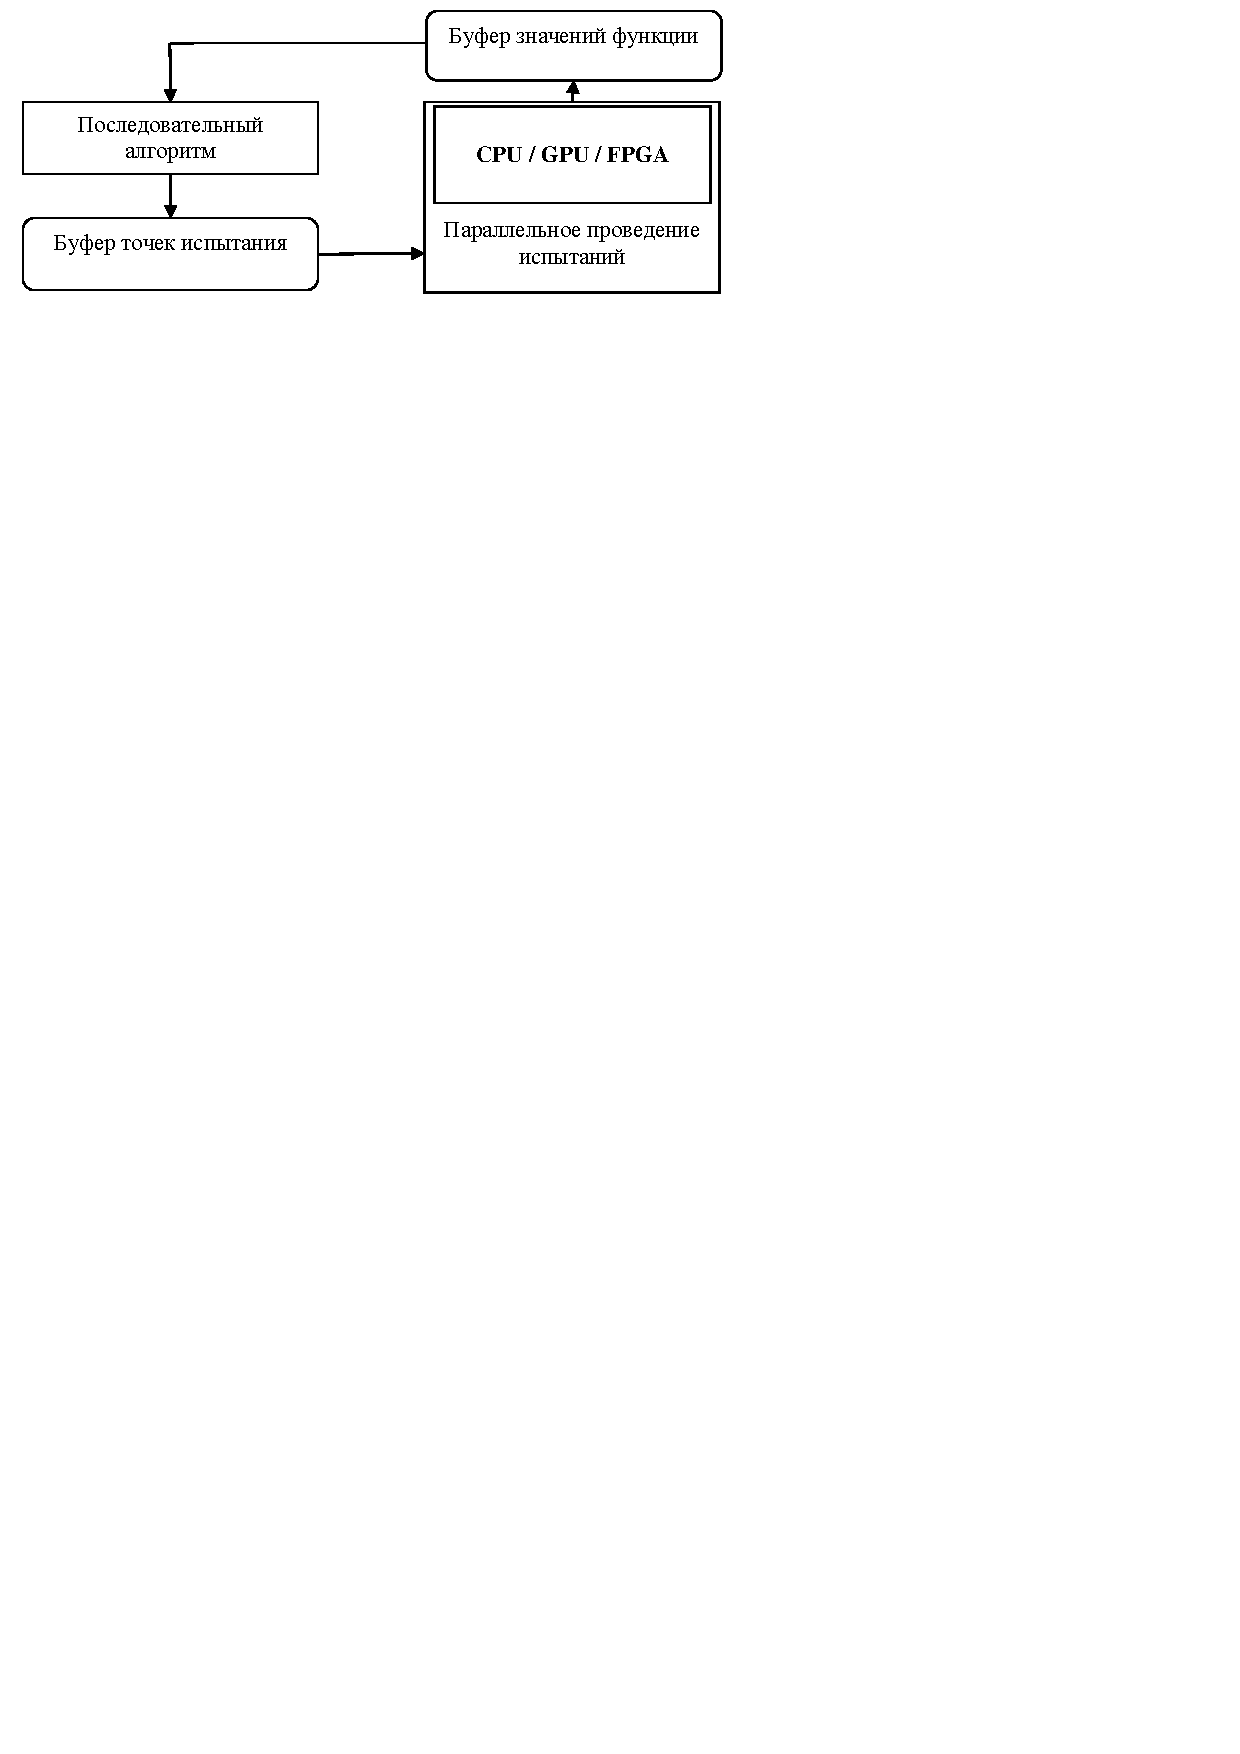
\includegraphics[width=0.7\linewidth]{./pic/s1.pdf}
  \caption{Общая схема организации параллельных вычислений.}
  \label{fig:s1}  
\end{center}
\end{figure}


\section{Результаты численных экспериментов}

В рамках работы были проведены вычислительные эксперименты на персональном компьютере с процессором Intel Core i5-10600 3.3GHz, 32 GB оперативной памяти и встроенной графической картой Intel UHD Graphics 630. Для получения исполняемого программного кода использовался компилятор Intel oneAPI DPC++ 2021.1. Вычислительные эксперименты выполнялись с использованием разработанного программного комплекса Globalizer [\ref{rfa:rulit:lit14}, \ref{rfa:rulit:lit15}].

Большинство известных тестовых задач из области многомерной глобальной оптимизации характеризуются небольшим временем вычисления значений целевой функции. Из-за этого при проведении экспериментов бывает сложно понять с чем может быть связано относительно большое время выполнения параллельного алгоритма: с появившимися, сравнительно с последовательной версией, накладными расходами или причина в неэффективном распараллеливании. В реальных же задачах вычисление функции самая трудоемкая и время затратная операция, поэтому такой проблемы не возникает. 

Нами предлагается вычислительно трудоемкая модификация существующих тестовых задач, расчет целевой функции заключается в интегрировании исходной тестовой функции по части параметров. Для этого изначально порождается задача, размерность которой в два раза больше искомой. При вычислении значения функции, первые $N$ координат фиксируются, а по остальным производится численное интегрирование по области определения функции. Для интегрирования используется метод средних прямоугольников. 

\begin{equation}
\varphi \left( {{y}_{1}},\ldots ,{{y}_{N}}~ \right)=\underset{{{a}_{N+1}}}{\overset{{{b}_{N+1}}}{\mathop \int }}\,\underset{{{a}_{N+2}}}{\overset{{{b}_{N+2}}}{\mathop \int }}\,\ldots \underset{{{a}_{2N}}}{\overset{{{b}_{2N}}}{\mathop \int }}\,\psi \left( {{y}_{1}},\ldots ,{{y}_{N}},{{y}_{N+1}},~..,{{y}_{2N}}~ \right)~d{{y}_{N+1}}d{{y}_{N+2}}..d{{y}_{2N}}~= 
\end{equation}
\begin{displaymath}
\underset{{{i}_{1}}=0}{\overset{M-1}{\mathop \sum }}\,\underset{{{i}_{2=0}}}{\overset{M-1}{\mathop \sum }}\,..\underset{{{i}_{N}}=0}{\overset{M-1}{\mathop \sum }}\,\left( \left( \underset{j=1}{\overset{2N}{\mathop \prod }}\,{{h}_{j}} \right)\psi \left( {{y}_{1}},{{y}_{2}},~..,{{y}_{N}},~{{y}_{{{\left( N+1 \right)}_{{{i}_{1}}}}}},{{y}_{{{\left( N+2 \right)}_{{{i}_{2}}}}}}~,~..,{{y}_{{{\left( 2N \right)}_{{{i}_{N}}}}}} \right) \right),
\end{displaymath}
\begin{displaymath}
D=\left\{ y~\in ~{{R}^{2N}}:~{{a}_{i}}\le ~~{{y}_{i}}\le ~~{{b}_{i}},~1\le i\le 2N \right\},
\end{displaymath}
\begin{equation}
{{y}_{{{\left( N+k \right)}_{{{i}_{k}}}}}}={{a}_{k}}+{{i}_{k}}*{{h}_{k}}+\frac{{{h}_{k}}}{2},
\end{equation}
\begin{equation}
{{h}_{k}}=~\frac{{{b}_{k}}-~{{a}_{k}}}{M},
\end{equation}


	
где $M$ -- количество участков интегрирования по одной координате, а $\psi$ – исходная тестовая функция. Очевидно, чем больше значение $M$, тем больше проводится вычислений. Изменяя число узлов в сетке интегрирования по всем координатам или число участков по одной, можно регулировать время выполнения вычислений.


Вначале проведем вычислительные эксперименты на классической задаче – функции Растригина. Она задается простой формулой, сепарабельна и не имеет ограничений по размерности. 


\begin{equation}
\label{Rastrigin}
\psi \left( {{y}_{1}},\ldots ,{{y}_{2N}}~ \right)=~\underset{i=1}{\overset{2N}{\mathop \sum }}\,(y_{i}^{2}-10\cos \left( 2\pi {{y}_{i}} \right)+10),
\end{equation}

\begin{displaymath}
-2.2<y\_i<1.8~,~1\le i\le 2N.
\end{displaymath}


На рис. \ref{fig:s2} изображены линии уровня двухмерной функции Растригина (слева) и интегрированной четырехмерной функции Растригина (справа). Как можно видеть, новая функция не сильно отличается от двухмерного оригинала, и даже глобальный минимум остался прежним – точка (0, 0).

\begin{figure}
\begin{center}
  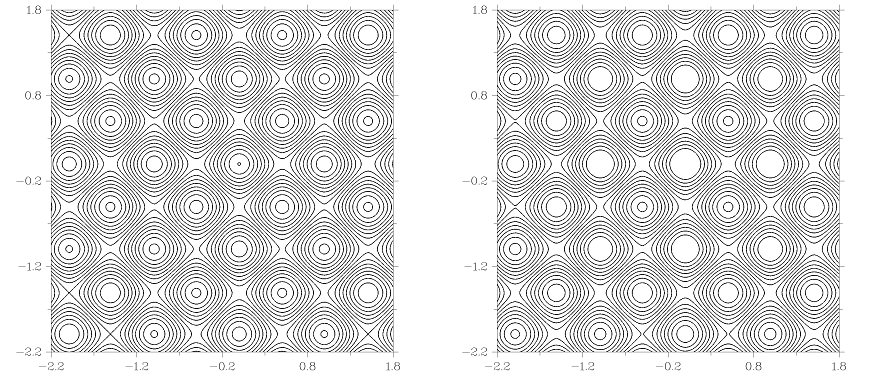
\includegraphics[width=1.0\linewidth]{./pic/s2.png}
  \caption{Линии уровня двумерной функции Растригина (слева) и интегрированной четырехмерной функции Растригина (справа).}
  \label{fig:s2}  
\end{center}
\end{figure}


Число итераций параллельного алгоритма глобального поиска (ПАГП) было ограничено 1000000, точность поиска $\varepsilon=0.01$ и параметр метода $r\ =\ 3$. Размерность задачи $N = 4$ и $5$. При вычислениях на CPU число потоков варьировалось от 1 до 8, а при вычислении на GPU от 256 до 1024. Использовался критерий остановки по попаданию в окрестность. В таблице \ref{table1} приведено число итераций ПАГП, в таблице \ref{table2} – ускорение по сравнению с однопоточным запуском.



\begin{table}[!ht]
    \centering
            \caption{Число итераций ПАГП при решении интегрированной функции Растригина.}
    \label{table1}
    \begin{tabular}{|l|l|l|l|l|l|l|l|l|}
    \hline
        N & CPU &   & ~ & ~ & ~ & GPU  & ~ & ~ \\ \hline
        ~ & P=1 & P=2 & P=4 & P=8 &   & P=256 & P=512 & P=1024  \\ \hline
        4 & 61231 & 26592 & 21007 & 6728 &   & 340 & 301 & 92  \\ \hline
        5 & 703548 & 328141 & 258351 & 99524 &   & 4642 & 2194 & 995  \\ \hline
    \end{tabular}
\end{table}



\begin{table}[!ht]
    \centering
            \caption{Ускорение ПАГП при решении интегрированной функции Растригина}
    \label{table2}
    \begin{tabular}{|l|l|l|l|l|l|l|l|}
    \hline
        N & CPU &   & ~ & ~ & GPU  & ~ & ~ \\ \hline
        ~ & P=2 & P=4 & P=8 & ~ & P=256 & P=512 & P=1024  \\ \hline
        4 & 2.1 & 2.1 & 5.6 & ~ & 2.8 & 3.1 & 9.4  \\ \hline
        5 & 1.9 & 2.0 & 4.3 & ~ & 2.4 & 4.9 & 9.7  \\ \hline
    \end{tabular}
\end{table}




Как можно видеть из полученных результатов, использование инструментов Intel oneAPI, при распараллеливании алгоритма глобального поиска, показала хорошие результаты на тестовой функции.

Далее проведем эксперименты на серии задач полученных интегрированием функций из генератора GKLS. Данный генератор описан в работах [\ref{rfa:rulit:lit16}, \ref{rfa:rulit:lit17}], дает возможность создавать серии задач многоэкстремальной оптимизации и заранее задавать их свойства, такие как: размерность задачи, количество локальных минимумов, размеры их областей притяжения, координата точки глобального минимума, значение функции в ней и т.п. На рис. \ref{fig:s3} изображены линии уровня двухмерной функции GKLS номер 9 (слева) и интегрированной функции GKLS номер 9, полученной интегрированием четырехмерной функции по последним двум параметрам (справа).

\begin{figure}
\begin{center}
  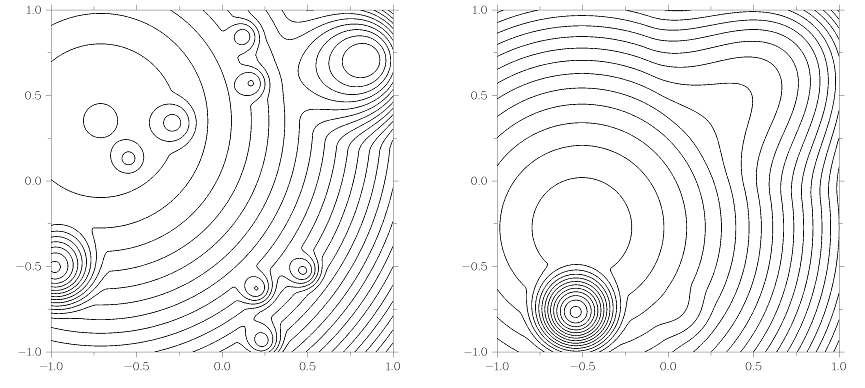
\includegraphics[width=1.0\linewidth]{./pic/s3.png}
  \caption{Функции GKLS (слева) и интегрированной функции GKLS (справа).}
  \label{fig:s3}  
\end{center}
\end{figure}

Число итераций ПАГП было ограничено 100000, точность поиска $\varepsilon=0.01$ и параметр метода $r\ =\ 4$. Размерность задачи $N = 4$ и 5. При вычислениях на CPU число потоков варьировалось от 1 до 8, а при вычислении на GPU от 256 до 1024. В таблице \ref{table3} приведено ускорение по сравнению с однопоточным запуском.

\begin{table}[!ht]
    \centering
    \caption{Ускорение ПАГП при решении серии интегрированных функций GKLS.}
    \label{table3}
    \begin{tabular}{|l|l|l|l|l|l|l|l|}
    \hline
        N & CPU &   & ~ & ~ & GPU  & ~ & ~ \\ \hline
        ~ & P=2 & P=4 & P=8 & ~ & P=256 & P=512 & P=1024  \\ \hline
        4 & 1.9 & 3.0 & 1.5 & ~ & 1.2 & 2.3 & 4.5  \\ \hline
        5 & 1.9 & 3.0 & 1.6 & ~ & 1.2 & 2.3 & 4.5  \\ \hline
    \end{tabular}
\end{table}



%=======================  Список литературы ==================================
%
% Команда \LITERRUS печатает "СПИСОК ЛИТЕРАТУРЫ" и обнуляет счетчики
%
\LITERRUS
% \rlitem{arg1}{arg2} --- создает пункт списка литературы.
% arg1 --- символическая ссылка на источник, используется при создании ссылки командой \ref
% arg2 --- текст, помещаемый в пункт списка. Может содержать команды выбора начертания 
%          символов и др.



\rlitem{rfa:rulit:lit1}{
\textit{Sergeyev Ya.D., Strongin R.G, Lera D.} Introduction to global optimization exploiting space-filling curves. Springer, 2013. 125 p.}

\rlitem{rfa:rulit:lit2}{
\textit{Strongin R.G., Sergeyev Ya.D.} Global Optimization with Non-convex Constraints. Sequential and Parallel Algorithms. Kluwer Academic Publishers, 2000. 704 p.}

\rlitem{rfa:rulit:lit3}{
\textit{Стронгин Р.Г., Гергель В.А., Гришагин В.А., Баркалов К.А.} Параллельные вычисления в задачах глобальной оптимизации. М.: Издательство Московского университета, 2013. 280 с.}

\rlitem{rfa:rulit:lit4}{
\textit{Pinter (Ed.), J.D.} Global Optimization: Scientific and Engineering Case Studies. Springer, 2006. 546 p.}

\rlitem{rfa:rulit:lit5}{
\textit{Стронгин Р.Г., Гергель В.А., Баркалов К.А.} Параллельные методы решения задач глобальной оптимизации. Известия высших учебных заведений. Приборостроение, 2009. Т. 52. № 10. С. 25 – 33.}

\rlitem{rfa:rulit:lit6}{
\textit{Захарова Е.М., Минашина И.К.} Обзор методов многомерной оптимизации. Информационные процессы, 2014. Т 14. №3. С. 256 – 274.}

\rlitem{rfa:rulit:lit7}{
\textit{Gaviano M., Lera D., Kvasov D.E., Sergeyev Y.D.} Software for generation of classes of test functions with known local and global minima for global optimization. ACM Transactions on Mathematical Software. – 2003. – Vol.  29. – P. 469-480.}


\rlitem{rfa:rulit:lit8}{
\textit{Сергеев Я.Д., Квасов Д.Е.} Диагональные методы глобальной оптимизации.  М.: Физматлит, 2008. – 352 c.}

\rlitem{rfa:rulit:lit9}{
\textit{Gablonsky J.M., Kelley C.T.} A Locally-Biased Form of the DIRECT Algorithm. Journal of Global Optimization, – 2001, Vol. 21, No. 1, – P. 27–37.}

\rlitem{rfa:rulit:lit10}{
\textit{Paulavicius R., Zilinskas J, Grothey A.} Parallel branch and bound for global optimization with combination of Lipschitz bounds. Optimization Methods \& Software,  2011. – Vol. 26, No. 3. P. 487–498.}

\rlitem{rfa:rulit:lit11}{
\textit{Боресков А.А., Харламов А.А., Марковский Н.Д., Микушин Д.Н., Мортиков Е.В., Мыльцев А.А., Сахарных Н.А., Фролов В.А.} Параллельные вычисления на GPU. Архитектура и программная модель CUDA. М.:  Издательство Московского университета, 2015. 336 с.}

\rlitem{rfa:rulit:lit12}{
\textit{Таненбаум Э., Остин Т.} Архитектура компьютера / перевод с английского Е. Матвеева. — 6-е изд. — Санкт-Петербург [и др.]: Питер, 2014. 816 с.}

\rlitem{rfa:rulit:lit13}{
\textit{Комолов Д.А., Мяльк Р.А., Зобенко А.А., Филиппов А.С.} Системы автоматизированного проектирования фирмы Altera MAX+Plus II и Quartus II. Издательство РадиоСофт, 2002. 355 c.}

\rlitem{rfa:rulit:lit14}{
\textit{Gergel V.P., Barkalov K.A., Sysoyev A.V.} A novel supercomputer software system for solving time-consuming global optimization problems. Numerical Algebra, Control and Optimization, 2018. Vol. 8, No. 1. P. 47-62.}

\rlitem{rfa:rulit:lit15}{
\textit{Sysoyev, A., Barkalov, K., Sovrasov, V., Lebedev, I., Gergel, V.} AGS NLP solver. \url{ https://github.com/sovrasov/ags_nlp_solver}}

\rlitem{rfa:rulit:lit16}{
\textit{Сергеев, Я.Д., Квасов Д.Е.} Диагональные методы глобальной оптимизации. М.: Физматлит, 2008. 352 c.}

%\rlitem{rfa:rulit:lit17}{
%\textit{Gaviano, M., Lera D., Kvasov D.E., Sergeyev Y.D.} Software for generation of classes of test functions with known local and global minima for global optimization/ M. Gaviano, D. Lera, D. E. Kvasov, Y. D. Sergeyev // ACM Transactions on Mathematical Software, 2003. Vol. 29. P. 469-480.}





%=======================  Список литературы ==================================
\medskip
\DateRU 

\medskip

\MakeAuthorsInfoRU

%===========================  REFERENCES =====================================
\pagebreak

\REFERENCES

\elitem{rfa:rulit:lit1}{
\textit{Sergeyev Ya.D., Strongin R.G, Lera D.} Introduction to global optimization exploiting space-filling curves. Springer, 2013. 125 p.}

\elitem{rfa:rulit:lit2}{
\textit{Strongin R.G., Sergeyev Ya.D.} Global Optimization with Non-convex Constraints. Sequential and Parallel Algorithms. Kluwer Academic Publishers, 2000. 704 p.}

\elitem{rfa:rulit:lit3}{
\textit{Strongin R.G., Gergel V.A., Grishagin V.A., Barkalov K.A.} %Параллельные вычисления в задачах глобальной оптимизации. М.: Издательство Московского университета, 2013. 280 с.
}

\elitem{rfa:rulit:lit4}{
\textit{Pinter (Ed.), J.D.} Global Optimization: Scientific and Engineering Case Studies. Springer, 2006. 546 p.}

\elitem{rfa:rulit:lit5}{
\textit{Strongin R.G., Gergel V.A., Barkalov K.A.} %Параллельные методы решения задач глобальной оптимизации. Известия высших учебных заведений. Приборостроение, 2009. Т. 52. № 10. С. 25 – 33.
}

\elitem{rfa:rulit:lit6}{
\textit{Zakharova E.M., Minashina I.K.} %Обзор методов многомерной оптимизации. Информационные процессы, 2014. Т 14. №3. С. 256 – 274.
}

\elitem{rfa:rulit:lit7}{
\textit{Gaviano M., Lera D., Kvasov D.E., Sergeyev Y.D.} Software for generation of classes of test functions with known local and global minima for global optimization. ACM Transactions on Mathematical Software. – 2003. – Vol.  29. – P. 469-480.}


\elitem{rfa:rulit:lit8}{
\textit{Sergeev Ya.D., Kvasov D.E.} %Диагональные методы глобальной оптимизации.  М.: Физматлит, 2008. – 352 c.
}

\elitem{rfa:rulit:lit9}{
\textit{Gablonsky J.M., Kelley C.T.} A Locally-Biased Form of the DIRECT Algorithm. Journal of Global Optimization, – 2001, Vol. 21, No. 1, – P. 27–37.}

\elitem{rfa:rulit:lit10}{
\textit{Paulavicius R., Zilinskas J, Grothey A.} Parallel branch and bound for global optimization with combination of Lipschitz bounds. Optimization Methods \& Software,  2011. – Vol. 26, No. 3. P. 487–498.}

\elitem{rfa:rulit:lit11}{
\textit{Boreskov A.A., Kharlamov A.A., Markovsky N.D., Mikushin D.N., Mortikov E.V., Myltsev A.A., Sakharnykh N.A., Frolov V.A.} %Параллельные вычисления на GPU. Архитектура и программная модель CUDA. М.:  Издательство Московского университета, 2015. 336 с.
}

\elitem{rfa:rulit:lit12}{
\textit{Tanenbaum A., Austin T.} Structured computer organization }

\elitem{rfa:rulit:lit13}{
\textit{Komolov D.A., Myalk R.A., Zobenko A.A., Filippov A.S.} %Системы автоматизированного проектирования фирмы Altera MAX+Plus II и Quartus II. Издательство РадиоСофт, 2002. 355 c.
}

\elitem{rfa:rulit:lit14}{
\textit{Gergel V.P., Barkalov K.A., Sysoyev A.V.} A novel supercomputer software system for solving time-consuming global optimization problems. Numerical Algebra, Control and Optimization, 2018. Vol. 8, No. 1. P. 47-62.}

\elitem{rfa:rulit:lit15}{
\textit{Sysoyev, A., Barkalov, K., Sovrasov, V., Lebedev, I., Gergel, V.} AGS NLP solver. \url{ https://github.com/sovrasov/ags_nlp_solver}}

\elitem{rfa:rulit:lit16}{
\textit{Sergeev, Ya.D., Kvasov D.E.} %Диагональные методы глобальной оптимизации. М.: Физматлит, 2008. 352 c.
}


\medskip
\DateEN

\bigskip

\MakeAuthorsInfoEN

%\end{document}
%============================ КОНЕЦ СТАТЬИ ==================================




\end{document}

